\chapter{Interactive Fashion Outfit Recommendation}
\label{sq:task}

\begin{figure*}[t]
  \centering
  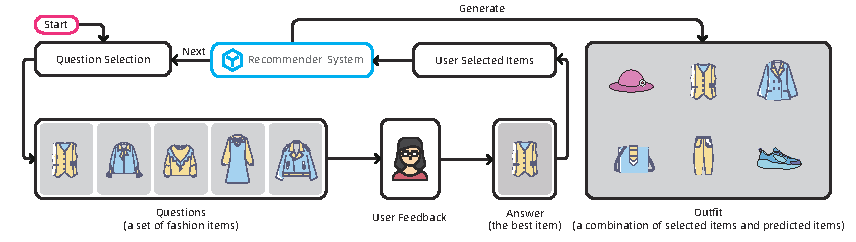
\includegraphics[width=\linewidth]{figures/workflow.pdf}
  \caption{The workflow of the interactive fashion outfit recommender system. 
  The recommender system composes and presents a question comprised of several fashion items.
The user responds to the question by selecting the best item from the presented fashion items.
After several rounds of question, the system is expected to recommend outfits 
that include the selected items and meet the user's preferences.}
  \label{workflow}
\end{figure*}


In this section, we describe the workflow of an interactive fashion outfit recommender system 
and provide the details of the interactive fashion outfit recommendation task.

\section{Definition}

Suppose we have a collection $I$ consisting $n$ different fashion items, i.e., $I = \left\{i_1, i_2, \ldots, i_n \right\}$. 
Each fashion item from the collection belongs to a category, e.g., tops, bottoms and dresses etc. 
The category of a specific item should be one of $C = \left\{c_1, c_2, \ldots, c_m\right\}$, where $C$ is the collection of all categories and $m$ denotes the number of categories. 
The item collection $I$ can be split to $m$ disjoint subsets of different categories, 
i.e., $I = I_{c_1} \cup I_{c_2} \cup \cdots \cup I_{c_m}$.

A question is defined as a set of fashion items and is used to let the user choose from multiple items.
To be comparable each other, fashion items in a question are to belong to the same category.
Thus, a question is defined as $Q = \left\{ i_1, i_2, \ldots, i_k \right\}$ 
and is a subset of $I_c$ of a certain category $c$ ($k$ is the number of items in a question). 

Similarly, outfit $O$ is defined as a set of items, i.e., $O \subset I$. 
In contrast to the question $Q$, $O$ contains items of different categories to form a complete outfit.


\section{Workflow}

Figure \ref{workflow} illustrates the overall workflow of the interactive fashion outfit recommendation system. 
The recommender system composes and presents a question consisting of multiple fashion items.
The user answers the question by choosing the best item from the set of fashion items.
After several rounds of question-answering, the system is expected to recommend outfits 
that include selected items and meet the user's preference.

The interactive fashion outfit recommender system must be able to provide {\it good} questions
for effectively estimating the user's preference,
and to recommend outfits compatible with fashion items given as answers to the questions. 
While the outfit recommendation component can be any existing models proposed in the literature (e.g., \cite{lin2020outfitnet}),
designing a question selection algorithm is an interesting challenge specific to this task. 
Since items selected by the user in the previous rounds matter to the question selection in the next round, 
the question selection algorithm should be able to identify questions that
facilitate the following interactions and achieve high accuracy in the outfit recommendation.

\section{Task}
Having described the workflow of the interactive fashion outfit recommender system,
we formally define the task of the interactive fashion outfit recommendation.

There are three main components in this task: the user $U$, question selection algorithm $S$,
and outfit recommendation algorithm $R$.
The user is a function that returns an item for a given question:
$U: Q \mapsto i$ where $i \in Q$.
Given a question-answering history up to time step $t$, $H_t=\left\{(Q_1, a_1), (Q_2, a_2), \ldots, (Q_t, a_t)\right\}$,
the question selection algorithm returns a question based on $H_t$, i.e., $S: H_t \mapsto Q$.
The outfit recommendation algorithm is a function that,
given the question-answering history $H_t$ and outfit $O$,
returns a score of $O$ with respect to $H_t$.
A set of outfits are then ranked by the score in descending order,
i.e., $R(H_t, O_a) < R(H_t, O_b) \Rightarrow O_a \prec O_b$ 
where $\prec$ represents the order in the outfit ranking.

With those main components, at each time step $t$, a question is given by $Q_t = S(H_{t-1})$.
The answer at time $t$ is given as follows: $a_t = U(Q_t)$.
After $T$ rounds of interactions, the system obtains the question-answering history $H_T$,
and recommends outfits ranked by $R$.
The outfit ranking can be evaluated in terms of any retrieval or recommendation effectiveness measures
such as HIT and nDCG.

As the user $U$ is out of score of the system, the goal of this task is to design effective functions for 
the question selection algorithm $S$ and outfit recommendation algorithm $R$
to achieve better performances in terms of some effectiveness measures.
Although one can address both simultaneously,
this work primarily focuses on the case where $R$ is given.
Therefore, our primary task is,
given user $U$ and outfit recommendation algorithm $R$,
to find the question selection algorithm $S$ that can achieve better performances
in the outfit recommendation.

For simplicity, we focus on a special case of this task
where the question selection algorithm $S$ is defined by a question value function $V$:
\begin{eqnarray}
S(H_t) = V(H_T, Q)
\label{eq:question_value}
\end{eqnarray}
where $V$ is a function that measure the value of the question $Q$ given the question-answering history $H_T$ of $T$ interactions,
and $\mathcal{Q}$ is a set of candidate questions. 
This simplification enables us to focus on measuring the goodness of questions and is suitable for the dataset explained in the next section.